\documentclass[12pt]{report}
\usepackage{subfigure}
\usepackage{amsmath,amssymb,array,bm,caption,fancyhdr,float,graphicx,indentfirst,parskip,siunitx,url,vmargin}
\usepackage[style=numeric]{biblatex}
\usepackage[english]{babel}
\usepackage[nottoc]{tocbibind}
\graphicspath{{images/}}
\addbibresource{project.bib}
\captionsetup[table]{labelsep=period}
\captionsetup[figure]{labelsep=period}
\begin{document}
\setlength{\parindent}{1em}
\vspace*{0.25cm}
\hrulefill
\thispagestyle{empty}
\begin{center}
    \begin{large}
        \sc{UM--SJTU Joint Institute
        \vspace{0.3em}\\
        A Perfect Pendulum
        \vspace{0.3em}\\
        VV285 Project
        \vspace{0.3em}\\}
    \end{large}
    \hrulefill
    \vspace*{5cm}\\
    \begin{large}
        \sc{Project Group 12}
    \end{large}
\end{center}
\vfill
\begin{large}
    \sc{Group Members:}
\end{large}
\begin{table}[h!]
    \flushleft
    \begin{tabular}{ll}
        An Ziying \hspace*{3em}&518370910139\hspace*{3em}\\
        Liu Yihua \hspace*{3em}&518021910998\hspace*{3em}\\
        Qiang Chenda \hspace*{3em}&518370910218\hspace*{3em}\\
        Xia Taoyue \hspace*{3em}&518370910087\hspace*{3em}\\
        Zhu Xingyu \hspace*{3em}&518370910023\hspace*{3em}\\
        \\
        Date: \today
    \end{tabular}
\end{table}
\newpage
\begin{abstract}
\setlength{\parindent}{0pt} \setlength{\parskip}{1.5ex plus 0.5ex minus 0.2ex}
    The objective of this project is to study simple pendulum and construct a strictly isochronous pendulum. We start our work from a basic mathematical pendulum. In this part, we initially recall the theorem of simple pendulums’ period and verify it by conducting an experiment and having mathematical calculations. Through the experiment result, we figure out the impact of the initial displacement of the pendulum.
    
	Based on the result, we further study how to make the period of a single pendulum independent of its initial displacement. Finally, we calculate and construct a Huygens pendulum that is absolutely isochronous.
\end{abstract}
\renewcommand{\thesection}{\arabic{section}}
\section{Introduction}
\subsection*{Objectives}
\begin{itemize}
    \item{Calculate the relationship between the initial displacement and the period of a single pendulum mathematically.}
    \item{Conduct an experiment to verify our calculation result.}
    \item{Calculate and construct a tautochronous pendulum.}
\end{itemize}
\subsection*{Background}
Pendulum has always been a common physical model. It is simple and is often used to keep time. A pendulum is an object that swings back and forth around a suspension point, and its period is generally closely related to the shape, size and mass distribution of the object.

Mathematical pendulum is one of the simplest pendulum in particle vibration system. If a particle is tied to one end of a string that cannot be extended and the other end is fixed, it is called a simple pendulum or mathematical pendulum. For the small amplitude oscillation (inclination angle is less than 5°) of a single pendulum, we usually regard it as the simple harmonic oscillation, whose period T is heavily related to the length l and the gravitational acceleration g, but not related to its initial displacement and the mass of the object \cite{Arnold1990}.
\begin{figure}[H]
    \centering
    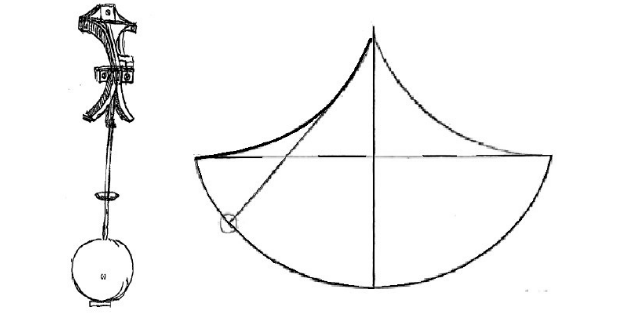
\includegraphics[width=0.8\linewidth]{1.png}
    \caption{Involute and isochronal pendulum \cite{Wu2012}.}
\end{figure}
However, the basic formula of period only applies to oscillations at very small angles. When the amplitude is large, the initial position of the pendulum will have a great influence on the period, thus affecting the accuracy of timing. Therefore, the absolute isochronous pendulum needs to be constructed by improving the structure of single pendulum. Christian Huygens found that when the trajectory of the mass center of the pendulum was the wheel line, the single pendulum would be isochronous. So he built the earliest isochronous pendulums by changing the length of their cycloids by adding plates with specific curves on either side of the pendulum.
\section{Experiment on the Period of the Pendulum}
\subsection{Theoretical Background of the Experiment}
In this experiment we make several trials with the pendulum.

By the equation:
\begin{equation*}
    T=2\pi\sqrt{\dfrac{l}{g}}(1-\dfrac{\theta_0^2}{16})
\end{equation*}
We can see that the period of the pendulum depends on the length of the string and the initial tilt angle.
\subsection{Apparatus}
The pendulum we use is like the photo above. There is a screw on top of the equipment which is used to adjust the length of the string.

What’s more, an iron ball is hung at the tail of the string to move in the trajectory of a circular arc.

A ruler and an angle gauge is used to measure the string length and the tilt angle.
\begin{figure}[H]
    \centering
    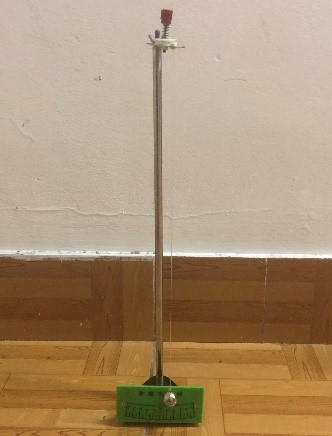
\includegraphics[width=0.7\linewidth]{3.jpg}
    \caption{Apparatus.}
\end{figure}
\subsection{Procedure}
First, we control the tilt angle to be the same, so that we can get the relation between period and string length.

We define the initial angle to be $45^\circ$ and adjust the string length. Then we release the ball and begin to take the period when it pass the equilibrium point the second time.

We take 10 periods to minimize the error.

Then we make another trial on the relation between the period and the initial tilt angle by control the string length at the same.

Fix the screw on the top to fix the string length. Then change the initial angle to release the ball.

\subsection{Results and Calculations of the Experiment}
The table below shows the relation between period and string length by making the angle the same.
\begin{table}[H]
        \centering
        \begin{tabular}{|c|c|c|c|c|}
                \hline
                Measurements & $\theta[^\circ]\ \pm\ 1[^\circ]$ & $L$[m]$\ \pm\ $0.01[m] & 10$T$[s]$\ \pm\ $0.01[s] &$u_T$ [s]\\
                \hline
                1 & 45 & 0.54 & 14.91 & 3$\times10^{-3}$\\
                \hline
                2 & 45 & 0.58 & 15.18 & 3$\times10^{-3}$\\
                \hline
                3 & 45 & 0.60 & 15.86 & 3$\times10^{-3}$\\
                \hline
                4 & 45 & 0.68 & 16.30 & 3$\times10^{-3}$\\
                \hline
                5 & 45 & 0.70 & 16.88 & 3$\times10^{-3}$\\
                \hline
                6 & 45 & 0.72 & 16.95 & 3$\times10^{-3}$\\
                \hline
        \end{tabular}
        \caption{Period vs. length.}
\end{table}
The table below shows the relation between period and angle.
\begin{table}[H]
        \centering
        \begin{tabular}{|c|c|c|c|c|}
                \hline
                Measurements & $L$[m]$\ \pm\ $0.01[m] & $\theta[^\circ]\ \pm1\ [^\circ]$ & 10$T$[s]$\pm$0.01[s] &$u_T$ [s]\\
                \hline
                1 & 0.60 & 15 & 15.18 & 9$\times10^{-4}$\\
                \hline
                2 & 0.60 & 30 & 15.53 & 1.8$\times10^{-3}$\\
                \hline
                3 & 0.60 & 45 & 15.58 & 3$\times10^{-3}$\\
                \hline
                4 & 0.60 & 60 & 15.78 & 4$\times10^{-3}$\\
                \hline
                5 & 0.60 & 75 & 15.93 & 4$\times10^{-3}$\\
                \hline
                6 & 0.60 & 90 & 16.07 & 5$\times10^{-3}$\\
                \hline
        \end{tabular}
        \caption{Period vs. $\theta_0$.}
\end{table}
Using \textsc{Origin}$^{\circledR}$ 2019b, we can calculate the Pearson's r of $T-\theta$ relationship is equal to 0.9819 and the Pearson's r of $T-l$ relationship is equal to 0.97652.
\subsection{Conclusion of the Experiment}
In conclusion, the period of the pendulum and the angle between the releasing position and the vertical line has a strong correlation. Besides, the period is also strongly correlated to the length of the string.
\section{Results and Calculation}
\subsection{The Pendulum Equation}
A mathematical pendulum of length $l$ and mass $m$ is a particle of mass $m$ joined by a weightless rod or thread of length $l$ with one end fixed on a support and the other end free rotating or oscillating in a plane due to gravity. A physical pendulum, however, is just a rigid body with mass $m$ that can swing freely suspending from a certain pivot. The difference to a physical pendulum is that the distance between the center of mass and the axis of suspension in a physical pendulum is comparable to the dimensions of the oscillating mass \cite{Awrejcewicz2012}. We denote the angle that the pendulum swings away from vertical as $\theta$, then by the definition of mechanical energy, we have
\begin{equation}
    E=K+U
\end{equation}
where K is the kinetic energy and U is the potential energy. By the theorem of kinetic energy and the equality $v=l\frac{\mathrm{d}\theta}{\mathrm{d}t}$, we have
\begin{equation}
    K=\frac{1}{2}mv^2=\frac{1}{2}ml^2{\dot{\theta}}^2
\end{equation}

Assuming the horizontal plane that lowest point falls has zero potential energy, then the potential energy of the system is
\begin{equation}
    U=mgh=mgl(1-\cos{\theta})
\end{equation}

Hence, the energy of a mathematical pendulum is given by
\begin{equation}
    E(\theta,\dot{\theta})=\frac{1}{2}ml^2{\dot{\theta}}^2+mgl(1-\cos{\theta})
\end{equation}
where $\dot{\theta}$ is the derivative $\frac{\mathrm{d}\theta}{\mathrm{d}t}$ and $g$ is the gravitational acceleration. Differentiating Eq. (4) of both $\theta$ and $\dot{\theta}$, the left hand side is equal to 0 because during the motion of the mathematical pendulum the mechanical energy is a constant according to the conservation law of mechanical energy. For the right hand side, the derivative at $\theta$ is $mgl\sin{\theta}$ and the derivative at $\dot{\theta}$ is $ml^2\ddot{\theta}$. Hence, we have
\begin{equation}
    \dfrac{\mathrm{d}^2\theta(t)}{\mathrm{d}t^2}+\dfrac{g}{l}\sin(\theta(t))=0
\end{equation}
\subsection{The Period of Mathematical Pendulum}
We release the pendulum at time $t=0$ and angle $\theta{0}=\theta_0$. To find out its period, we first consider the geometric relationship
\begin{equation}
    h=l(\cos{\theta}-\cos{\theta_0})
\end{equation}
we have
\begin{equation}
    \left|\dot{\theta}\right|=\dfrac{\sqrt{2gh}}{l}
\end{equation}
Besides, by the conservation of mechanical energy
\begin{equation}
    \dfrac{1}{2}mv^2=\dfrac{1}{2}ml^2\dot{\theta}^2=mgh
\end{equation}
we have
\begin{equation}
    \left|\dot{\theta}\right|=\sqrt{\dfrac{2g}{l}(\cos{\theta}-\cos{\theta_0})}
\end{equation}

For a single period, the map $t\mapsto\theta$ is bijective and therefore invertible. By the Inverse Function Theorem, consider the inverse function
\begin{equation}
    \dfrac{\mathrm{d}t}{\mathrm{d}\theta}=\sqrt{\dfrac{l}{2g}}\dfrac{1}{\cos{\theta}-\cos{\theta_0}}
\end{equation}
Integrating Eq. (10) from $\theta_0$ to $-\theta_0$ to $\theta_0$, equaling to integrating from 0 to $\theta_0$ for four times,
\begin{equation}
    T=4\sqrt{\dfrac{l}{2g}}\int_0^{\theta_0}\dfrac{\mathrm{d}\theta}{\sqrt{\cos{\theta}-\cos{\theta_0}}}
\end{equation}
Using the substitution
\begin{equation}
    \phi=\arcsin{\dfrac{\sin{\dfrac{\theta}{2}}}{\sin\dfrac{\theta_0}{2}}}
\end{equation}
Since $\dfrac{\mathrm{d}\arcsin{x}}{\mathrm{d}x}=\dfrac{1}{\sqrt{1-x^2}}$ and $\cos{\theta}=1-2\sin^2{\dfrac{\theta}{2}}$, we have
\begin{equation}
    \mathrm{d}\phi=\dfrac{\cos{\dfrac{\theta}{2}}\mathrm{d}\theta}{2\sqrt{\sin^2{\dfrac{\theta_0}{2}}-\sin^2{\dfrac{\theta}{2}}}}
\end{equation}
Plugging Eq. (13) into Eq. (11),
\begin{equation}
    \begin{split}
        T=2\sqrt{\dfrac{l}{g}}\int_{0}^{\theta_0}\dfrac{\mathrm{d}\theta}{\sqrt{\sin^2{\dfrac{\theta_0}{2}}-\sin^2{\dfrac{\theta}{2}}}}=4\sqrt{\dfrac{l}{g}}\int_{0}^{\pi/2}\dfrac{\mathrm{d}\phi}{\cos\dfrac{\theta}{2}}\\=4\sqrt{\dfrac{l}{g}}\int_{0}^{\pi/2}\dfrac{\mathrm{d}\phi}{\sqrt{1-\sin^2{(\theta_0/2)}\sin^2{\phi}}}
    \end{split}
\end{equation}
We first want to show the integral-form expression of the arithmetic-geometric mean $M(x,y)$. Consider the so-called complete elliptic integral of the first kind,
\begin{equation}
    T(a,b)=\dfrac{2}{\pi}\int_0^{\pi/2}\dfrac{\mathrm{d}\theta}{\sqrt{a^2\cos^2{\theta}+b^2\sin^2{\theta}}}
\end{equation}
Substitute $t:=b\tan{\theta}$ and $\mathrm{d}t=b/\cos^2{\theta}$ we have
\begin{equation}
    T(a,b)=\dfrac{1}{\pi}\int_{-\infty}^{\infty}\sqrt{\dfrac{\cos^4{\theta}}{b^2(a^2\cos^2{\theta}+b^2\sin^2{\theta})}}\mathrm{d}t=\dfrac{1}{\pi}\int_{-\infty}^{\infty}\dfrac{\mathrm{d}t}{\sqrt{(a^2+t^2)(b^2+t^2)}}
\end{equation}
Substitute $u:=(t-ab/t)/2$ and $\mathrm{d}u=(1+ab/t^2)/2$ we have
\begin{equation}
    T(a,b)=\dfrac{1}{\pi}\int_{-\infty}^{\infty}\dfrac{\mathrm{d}u}{\sqrt{((\dfrac{a+b}{2})^2+u^2)(ab+u^2)}}
\end{equation}
Denote the arithmetic-geometric mean of $a,b\in\mathbb{R}$ as $M(a,b)$, then we have the relationship
\begin{equation}
    T(a,b)=\dfrac{1}{M(a,b)}
\end{equation}
By Eq. (14) and Eq. (15), letting $\theta$ in Eq. (15) be $\phi$ in Eq. (14), the formula relating the period of the pendulum to the arithmetic-geometric mean is
\begin{equation}
    T=2\pi\sqrt{\dfrac{l}{g}}\cdot\dfrac{2}{\pi}\int_{0}^{\pi/2}\dfrac{\mathrm{d}\phi}{\cos^2{\phi}+\cos^2\dfrac{\theta_0}{2}\sin^2{\phi}}=\dfrac{2\pi}{M(1,\cos{\dfrac{\theta_0}{2}})}\sqrt{\dfrac{l}{g}}
\end{equation}
Take $M(a,b)=(a+b)/2$,
\begin{equation}
    T=\dfrac{4\pi}{1+\cos{\dfrac{\theta_0}{2}}}\sqrt{\dfrac{l}{g}}
\end{equation}
Since $\dfrac{1+\cos(\theta_0/2)}{2}=\cos^2{\dfrac{\theta_0}{4}}$,
\begin{equation}
    T=2\pi\sec^2{\dfrac{\theta_0}{4}}\sqrt{\dfrac{l}{g}}
\end{equation}
Using Maclaurin series expansion we write the Legendre polynomial solution,
\begin{equation}
    \sec^2{\dfrac{\theta_0}{4}}=1+\dfrac{1}{16}\theta_0^2+\cdots
\end{equation}
Since $\theta_0$ is infinitesimal, the period is approximately given by
\begin{equation}
    T\approx 2\pi\sqrt{\dfrac{l}{g}}(1+\dfrac{\theta_0^2}{16})\approx 2\pi\sqrt{\dfrac{l}{g}}
\end{equation}
\subsection{The Relation Between the Potential Energy and Its Derivative of a Tautochrone}
According to the conservation of energy, i.e., the total energy is equal to the potential energy plus the kinetic energy. Hence, we have
\begin{equation}
    U(\gamma(t))+\dfrac{m}{2}\gamma^{'}(t)^2=\rm{const}.
\end{equation}
At the initial point, $t=0$, $\gamma(t)=x_1$, which is the initial displacement. Also, the initial velocity of the object is 0, so $\gamma^{'}(0)=0$. Substitute them into the energy equation, we have
\begin{equation}
    U(x_1)=U(\gamma(0))=\rm{const}.
\end{equation}
Since the velocity is equal to $\gamma^{'}(t)$, we deduce from Eq. (24) that
\begin{equation}
    \gamma^{'}(t)=\sqrt{\dfrac{2}{m}(U(x_1)-U(x))}
\end{equation}
For a small interval of time,
\begin{equation}
    \mathrm{d}t=\dfrac{\mathrm{d}s}{v}
\end{equation}
Integrating Eq. (27), we have
\begin{equation}
    T(x_1)=\int_0^T\mathrm{d}t=\int_0^{x_1}\dfrac{1}{v}\mathrm{d}s=\sqrt{\dfrac{m}{2}}\int_0^{x_1}\dfrac{1}{\sqrt{U(x_1)-U(x)}}\mathrm{d}x
\end{equation}
To substitute Eq. (28), we consider
\begin{equation}
    y^2=\dfrac{U(x)}{U(x_1)}
\end{equation}
Differentiating the square root of Eq. (29), we have
\begin{equation}
    \dfrac{\mathrm{d}y}{\mathrm{d}x}=\dfrac{U^{'}(x)}{2\sqrt{U(x)U(x_1)}}
\end{equation}
so the integral component of Eq. (28) can be written as
\begin{equation}
    \int_0^{x_1}\dfrac{\mathrm{d}x}{\sqrt{U(x_1)(1-\frac{U(x)}{U(x_1)})}}=\int_{0}^{1}\dfrac{2\sqrt{U(x)U(x_1)}\mathrm{d}y}{\sqrt{U(x_1)}\sqrt{1-y^2}U^{'}(x)}=\int_0^1\dfrac{2\sqrt{U(x)}}{U^{'}(x)\sqrt{1-y^2}}\mathrm{d}y
\end{equation}
where we use $x=U^{-1}[U(x_1)y^2]$ derived from Eq. (29). Hence, we can define
\begin{equation}
    T(x)=\sqrt{\dfrac{m}{2}}\int_0^1\dfrac{2\sqrt{U(x)}}{U^{'}(x)\sqrt{1-y^2}}\mathrm{d}y
\end{equation}

For fixed $y$, $x$ increases as $x_1$ increases, because $x=U^{-1}[U(x_1)y^2]$, where $U$ and $U_1$ are strictly increasing functions. If $T$ does not change as $x_1$ changes, it will obviously not change as $x$ changes, so $T^{'}(x)=0$. Denote
\begin{equation}
    H(x,y):=\int_0^1\dfrac{2\sqrt{U(x)}}{U^{'}(x)\sqrt{1-y^2}}\mathrm{d}y
\end{equation}
Differentiate $T(x)$, we have
\begin{equation}
    \mathrm{D}T(x)=\sqrt{\dfrac{m}{2}}\int_0^1\mathrm{D}H(\cdot,y)\mathrm{d}y=\sqrt{\dfrac{m}{2}}\int_0^1\left[\dfrac{\sqrt{U(x)}}{U^{'}(x)}\right]^{'}\cdot\dfrac{2}{\sqrt{1-y^2}}\mathrm{d}y
\end{equation}
Since $x$ can be kept independent of $y$ by changing $x_1$, we can continue to write the following equations
\begin{equation}
    \mathrm{D}T(x)=\sqrt{\dfrac{m}{2}}\left[\dfrac{\sqrt{U(x)}}{U^{'}(x)}\right]^{'}\int_0^1\dfrac{2}{\sqrt{1-y^2}}\mathrm{d}y
\end{equation}
Calculating the integral,
\begin{equation}
    \mathrm{D}T(x)=\pi\sqrt{\dfrac{m}{2}}\left[\dfrac{\sqrt{U(x)}}{U^{'}(x)}\right]^{'}=0
\end{equation}
Therefore, $\left[\dfrac{\sqrt{U(x)}}{U^{'}(x)}\right]^{'}=0$.

Since $U(x)>0$ and $U^{'}(x)>0$ for all $x\in\mathbb{R}$, we can state
\begin{equation}
    U^{'}(x)=c\sqrt{U(x)}\qquad(c>0)
\end{equation}
\subsection{The Relation Between the Path Length and the Acceleration of a Tautochrone}
Since we have the relationship $U^{'}(s)=c\sqrt{U(s)}$ in the previous subsection, we can write it as
\begin{equation}
    \dfrac{\mathrm{d}U}{\sqrt{U}}=c\cdot\mathrm{d}s
\end{equation}
Solving Eq. (38) as a differential equation by integrating both hand sides,
\begin{equation}
    \int\dfrac{\mathrm{d}U}{\sqrt{U}}=\int c\cdot\mathrm{d}s
\end{equation}
we have
\begin{equation}
    2\sqrt{U}+c_0=c\cdot s\qquad(c_0\in\mathbb{R})
\end{equation}
Since $U(0)=0$, we can get $c_0=0$. Therefore, we can get $U=\dfrac{c^2s^2}{4}$ from Eq. (40). According to Newton's Second Law of Motion,
\begin{equation}
    F=m\cdot a=m\dfrac{\mathrm{d}^2s}{\mathrm{d}t^2}
\end{equation}
where $m$ is the mass. From the property of the potential energy, a force of $F(s)=-U^{'}(s)$ is exerted on an object in the potential field. Since $c_0=0$, we deduce that
\begin{equation}
    F(s)=-U^{'}(s)=-\dfrac{c^2s}{2}
\end{equation}
Hence,
\begin{equation}
    \dfrac{\mathrm{d}^2s}{\mathrm{d}t^2}=a=\dfrac{F(s)}{2m}=-\dfrac{c^2s}{2m}
\end{equation}
from which we have the coefficient $k=\dfrac{c^2}{2m}$.

On the other hand, in the model of a simple pendulum as is shown in Figure 1, the force tangential to the trajectory is
\begin{equation}
    F=-mg\sin{\theta}
\end{equation}
\begin{figure}[H]
    \centering
    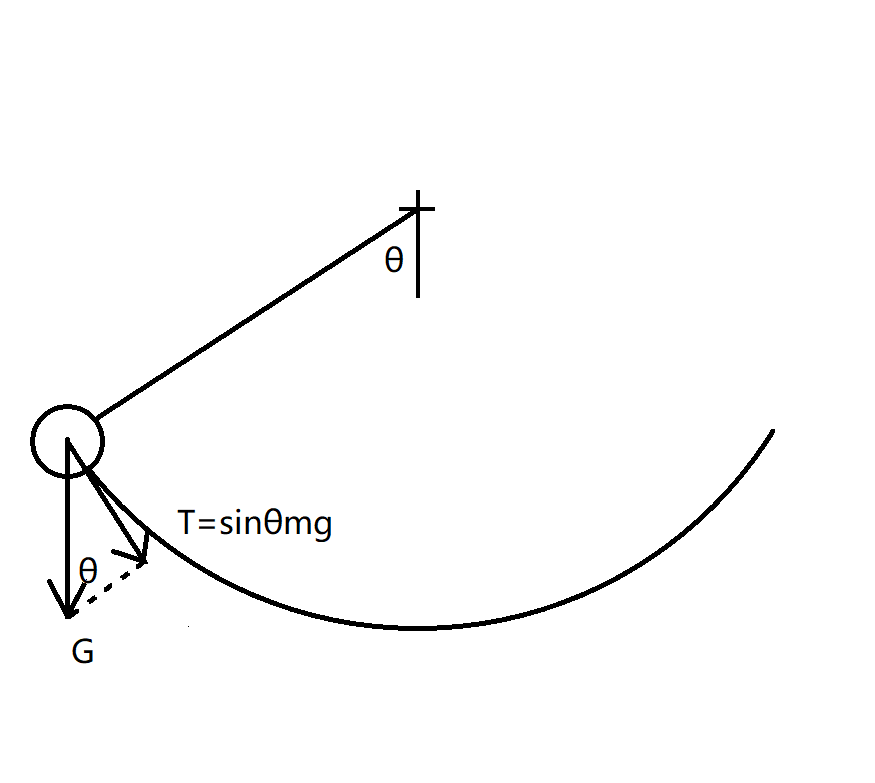
\includegraphics[width=0.8\linewidth]{2.png}
    \caption{Free body diagram of a pendulum constrained by plates.}
\end{figure}
Hence,
\begin{equation}
    \dfrac{\mathrm{d}^2s}{\mathrm{d}t^2}=a=\dfrac{F}{m}=-g\sin{\theta}
\end{equation}
Since $s=\theta\cdot l$, the coefficient is
\begin{equation}
    k(\theta)=\dfrac{\frac{\mathrm{d}^2s}{\mathrm{d}t^2}}{-s}=\dfrac{g\sin{\theta}}{\theta l}
\end{equation}
Differentiating $k$,
\begin{equation}
    k^{'}(\theta)=\dfrac{\theta\cos{\theta}-\sin{\theta}}{{\theta}^2}=\dfrac{\theta-\tan{\theta}}{\frac{{\theta}^2}{\cos{\theta}}}
\end{equation}
From Eq. (47) we know that $\tan{\theta}>\theta$ on the interval $\left(0,\dfrac{\pi}{2}\right)$ since $(\tan{\theta})^{'}=\sec^2{\theta}>1$, ${\theta}^{'}=1$, and $\tan{\theta}=\theta$ when $\theta=0$, so $k^{'}(\theta)<0$. Hence, $k$ is not a constant. Therefore, a simple pendulum does not satisfy the relation of
\begin{equation}
    \dfrac{\mathrm{d}^2s}{\mathrm{d}t^2}=-ks
\end{equation}
\subsection{A Cycloid Curve}
Given the equation $\frac{\mathrm{d}^2s}{\mathrm{d}t^2}=-ks$ from the previous subsection, now we want to show that this curve is a cycloid and give the parametric equations of this cycloid. Newton's Second Law of Motion gives us
\begin{equation}
    \dfrac{\mathrm{d}^2s}{\mathrm{d}t^2}=-g\sin{\theta}
\end{equation}
Combining these two equations Eq. (48) and Eq. (49), we have
\begin{equation}
    s=\dfrac{g\sin{\theta}}{k}
\end{equation}
Differentiate Eq. (50), we have
\begin{equation}
    \mathrm{d}s=\dfrac{g\cos{\theta}}{k}\mathrm{d}\theta
\end{equation}
On the other hand,
\begin{equation}
    \mathrm{d}s=\sqrt{\left(\frac{\mathrm{d}x}{t}\right)^2+\left(\frac{\mathrm{d}y}{t}\right)^2}\mathrm{d}\theta
\end{equation}
Since the normal component of the speed is 0,
\begin{equation}
    \dfrac{\mathrm{d}x}{\mathrm{d}t}\sin{\theta}=\dfrac{\mathrm{d}y}{\mathrm{d}t}\cos{\theta}
\end{equation}
Combining these two equations Eq. (51) and Eq. (52), we have $\mathrm{d}s=\mathrm{d}x/\cos{\theta}$. Write the time derivative,
\begin{equation}
    \dfrac{\mathrm{d}s}{\mathrm{d}{t}}=\dfrac{\mathrm{d}x}{\cos{\theta}\mathrm{d}t}
\end{equation}
Substitute Eq. (51) into Eq. (54), we have
\begin{equation}
    \dfrac{\mathrm{d}x}{\mathrm{d}{t}}=\dfrac{g}{2k}(1+\cos{2\theta})\dfrac{\mathrm{d}\theta}{\mathrm{d}{t}}
\end{equation}
From Eq. (53) we get
\begin{equation}
    \dfrac{\mathrm{d}y}{\mathrm{d}{t}}=\dfrac{g}{2k}\sin{2\theta}\dfrac{\mathrm{d}\theta}{\mathrm{d}{t}}
\end{equation}
Multiply both hand sides of Eq. (55) and Eq. (56) with $\mathrm{d}t$ and integrate both sides respectively, we get
\begin{equation}
    x=\int\mathrm{d}x=\int\dfrac{g}{2k}(1+\cos{2\theta})\mathrm{d}\theta=\dfrac{g}{4k}(2\theta+\sin{2\theta})+C_1
\end{equation}
\begin{equation}
    y=\int\mathrm{d}y=\int\dfrac{g}{2k}\sin(2\theta)\mathrm{d}\theta=-\dfrac{g}{4k}\cos{2\theta}+C_2
\end{equation}
Applying the initial conditions $x=0$ and $y=-g/(2k)$, both when $\theta=0$, we finally get
\begin{equation}
    x=\dfrac{g}{4k}(2\theta+\sin{2\theta})
\end{equation}
\begin{equation}
    y=-\dfrac{g}{4k}(\cos{2\theta}+1)
\end{equation}
Now we can know that such curve is a cycloid and the parametrization of this cycloid is given in Eq. (59) and Eq. (60).
\subsection{Description of the Construction of a Tautochronous Pendulum}
Then we want to further explore the construction of a tautochronous pendulum. From Eq. (55) and Eq. (56) we have
\begin{equation}
    (\mathrm{d}x)^2+(\mathrm{d}y)^2=\dfrac{g^2}{2k^2}(1+\cos{2\theta})(\mathrm{d}\theta)^2
\end{equation}
According to the conservation law of mechanical energy $\frac{1}{2}mv^2=mg|y|$, the velocity $v=\sqrt{2g|y|}$. Plugging into $v=\dfrac{\mathrm{d}s}{\mathrm{d}t}$,
\begin{equation}
    \mathrm{d}t=\dfrac{\mathrm{d}s}{\sqrt{2g|y|}}=\dfrac{\sqrt{(\mathrm{d}x)^2+(\mathrm{d}y)^2}}{\sqrt{2g|y|}}
\end{equation}
From Eq. (56) and Eq. (61), we can get
\begin{equation}
    \mathrm{d}t=\dfrac{\sqrt{\dfrac{g^2}{2k^2}(1+\cos{2\theta})}}{\sqrt{\dfrac{g^2}{2k}(1+\cos{2\theta})}}\mathrm{d}\theta=\dfrac{\mathrm{d}\theta}{\sqrt{k}}
\end{equation}
Integrate both hand sides,
\begin{equation}
    T=\int_0^{\pi}\dfrac{\mathrm{d}\theta}{\sqrt{k}}=\dfrac{\pi}{\sqrt{k}}
\end{equation}
Now considering an intermediate point $\theta_0$, by the conservation law of mechanical energy, $\frac{1}{2}mv^2=mgy=mgy_0$, so $v=\sqrt{2g(y-y_0)}$. Plugging into $v=\frac{\mathrm{d}s}{\mathrm{d}t}$,
\begin{equation}
    \mathrm{d}t=\dfrac{\mathrm{d}s}{2g(y-y_0)}=\dfrac{\sqrt{(\mathrm{d}x)^2+(\mathrm{d}y)^2}}{2g(y-y_0)}=\dfrac{\sqrt{\dfrac{g^2}{2k^2}(1+\cos{2\theta})}}{\sqrt{\left|-\dfrac{g^2}{2k}(1+\cos{2\theta}-1-\cos{2\theta_0})\right|}}\mathrm{d}\theta
\end{equation}
Then integrate both hand sides by computer software,
\begin{equation}
    T=\dfrac{\pi}{\sqrt{k}}
\end{equation}
which shows $T$ is the same for any point of the curve. Hence, the curve is a cycloid \cite{Weisstein2019}.
\section{Conclusion}
In this project we explored simple pendulum and isochronous pendulum.We began our project from the calculation about the period of mathematical pendulum. Base on the obtained result, we conducted an experiment and verified that the initial displacement do have certain effect on the oscillation period of the pendulum.

Besides, we further study how to make the period of a single pendulum independent of its initial displacement. By adding two plates on the sides, we altered the length of the pendulum to make it isochronous. Through calculation, we got the curve function of the plates and constructed a mathematical model of Huygens pendulum which is absolutely isochronous.

In the future research, we may continue this topic and exploring it further by building and analyzing the real Huygens pendulum to study how to make real pendulum isochronous, that is, to eliminate the influence of external factors such as the rotation of the earth.
\renewcommand\bibname{References}
\printbibliography
\end{document}